% Part: sets-functions-relations
% Chapter: infinite
% Section: hilberts-hotel
%
\documentclass[../../../include/open-logic-section]{subfiles}

\begin{document}

\olfileid{sfr}{infinite}{hilbert}
\olsection{హిల్బర్ట్ హోటల్}

సహజ సంఖ్యల సమితి అనంతమైనదని స్పష్టం. కాబట్టి సహజ సంఖ్యలను ముందే
\emph{ఉపయోగించుకోకుండా} ఉండాలంటే, సహజ సంఖ్యలను ప్రస్తావించాల్సిన
అవసరం లేని పదాల్లో అనంత సమితిని వర్ణించడం మన మొదటి మెట్టు కావాలి.
1924లో హిల్బర్ట్ ఇచ్చిన ఉపన్యాసంలో వివరించిన చక్కని విధానం ఇదిగో.
ఆయన మనల్ని ఇలా ఊహించమంటాడు:
\begin{quote}
[\ldots] పరిమిత సంఖ్యలో గదులు గల ఒక హోటల్. ఈ గదుల్లో ప్రతి
ఒక్కదానిలో సరిగ్గా ఒక అతిథి ఉండాలి. ఇప్పుడు అతిథులు తమ గదులను ఏదో
విధంగా మార్చుకున్నా, [కానీ] ప్రతి గదిలో ఇప్పటికీ ఒకరికంటే ఎక్కువ మంది
లేకుండా ఉంటే, ఏ గదీ ఖాళీ కాదు; ఈ విధంగా హోటల్ యజమాని కొత్తగా వచ్చిన
అతిథికి కొత్త స్థలాన్ని కల్పించలేడు [\ldots
\textparagraph \ldots]

ఇప్పుడు హోటల్‌కు $1$, $2$, $3$, $4$, $5$, \dots అని సంఖ్యలు గల
అనంత గదులు ఉన్నాయని, ప్రతి గదిలో సరిగ్గా ఒక అతిథి ఉన్నాడని
నిర్దేశిద్దాం. కొత్త అతిథి రాగానే యజమాని పాత అతిథుల్లో ప్రతి ఒక్కరినీ
వారి గది సంఖ్య కంటే ఒకటి ఎక్కువ సంఖ్య గల గదికి మార్చితే చాలు;
కొత్తగా వచ్చిన అతిథికి గది~$1$ ఖాళీ అవుతుంది.
	\begin{center}
		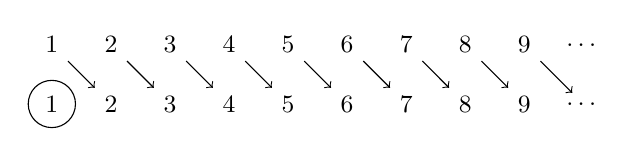
\begin{tikzpicture}[scale = .75]
		\foreach \x in {1, 2, 3, 4, 5, 6, 7, 8, 9}
		{
			\node (\x a) at (\x, 1) {\small{\x}};
			\node (\x b) at (\x, 2) {\small{\x}};
		}
		\node (dotsa) at (10, 1) {\small{\ldots}};
		\node (dotsb) at (10, 2) {\small{\ldots}};
		\draw[->] (1b)--(2a);
		\draw[->] (2b)--(3a);
		\draw[->] (3b)--(4a);
		\draw[->] (4b)--(5a);
		\draw[->] (5b)--(6a);
		\draw[->] (6b)--(7a);
		\draw[->] (7b)--(8a);
		\draw[->] (8b)--(9a);
		\draw[->] (9b)--(dotsa);
		\draw (1,1) circle (.4);
		\end{tikzpicture}
	\end{center}
	(\citealt[730]{EwaldSieg2013}లో ప్రచురించబడింది; అనువాదం మాది)
\end{quote}
కీలకమైన విషయం ఏమిటంటే, హిల్బర్ట్ హోటల్‌లో అనంత గదులు ఉన్నాయి;
దీన్ని చెప్పడం అంటే ఏమిటో నిర్వచించడానికి ఆయన వివరణను తీసుకోవచ్చు.
నిజానికి ఇదే డెడెకిండ్ విధానం (ఇక్కడ దీన్ని చాలా కాలభ్రంశంతో
వివరిస్తున్నాం; డెడెకిండ్ నిర్వచనం \citeyear{Dedekind1888} నాటిది):

\begin{defn}\ollabel{defn:DedekindInfinite}
$A$ నుంచి $A$ యొక్క ఒక క్రమ ఉపసమితికి \tetoken{ఒక ఒకటి-ఒకటి ప్రమేయం}{!!a{injection}} ఉన్నప్పుడు మాత్రమే
$A$ సమితిని \emph{డెడెకిండ్ అనంతం} అంటాం. అంటే, $o \notin \ran{f}$
అయ్యే ఏదో $o \in A$, అలాగే \tetoken{ఒక ఒకటి-ఒకటి ప్రమేయం}{!!a{injection}} $f \colon A \to A$ ఉన్నాయి.
\end{defn}

\end{document}
